\documentclass[twocolumn, 10pt]{article}

\usepackage{geometry}
\geometry{
	a4paper,
	total={6.85in, 9.92in},
	left=0.71in,
	top=0.63in,
}
\usepackage[utf8]{inputenc}
\usepackage{hyperref}
\usepackage{graphicx}
\usepackage{listings}
\usepackage{lipsum} % XXX: Remove that
\usepackage{newunicodechar}

% unicodes styling
% \DeclareUnicodeCharacter{2014}{\dash}
% unicodes - end
\pagenumbering{gobble}

% listing styling
\lstdefinestyle{c}{language=c,
    morekeywords={uint32_t, int32_t, uint8_t, printf, size_t},
        backgroundcolor=\color{clr-background},
        basicstyle=\color{clr-text}, % any text
        stringstyle=\color{clr-string},
        identifierstyle=\color{clr-variable}, % about not directive, comment, string or known type
        commentstyle=\color{clr-comment},
        directivestyle=\color{clr-preprocessor}, % preprocessor commands
        % listings doesn't differentiate between types and keywords (e.g. int vs return)
        % use the user types color
        keywordstyle=\color{clr-type},
        keywordstyle={[2]\color{clr-constant}}, % you'll need to define these or use a custom language
        tabsize=2
    frame=tb,
}
\lstdefinestyle{sh}{
    language=sh,
    basicstyle=\tiny\sffamily,
    numbers=left,
    % numberstyle=\tiny,
    % numbersep=3pt,
    frame=tb,
    columns=fullflexible,
        backgroundcolor=\color{clr-background},
}
\lstdefinestyle{json}{
    language=sh,
    basicstyle=\tiny\sffamily,
    numbers=left,
    % numberstyle=\tiny,
    % numbersep=3pt,
    frame=tb,
    columns=fullflexible,
        backgroundcolor=\color{clr-background},
}
% listing - end
\setlength{\parindent}{0pt}

\title{RPI4 remote debug recipe!}
\author{Kajetan Brzuszczak}

\makeatletter
\newcommand{\fsize}{\f@size pt }
\newcommand{\textFontName}{\f@family}
\renewcommand{\maketitle}{
\begin{flushleft}
{\noindent\Huge\bf\@title}\break
\end{flushleft}
}
\makeatother

\begin{document}
\maketitle

Tools: \textit{RPI4, C++, VSCode, CMake}

\subsection{Environment}
Project tree:
\begin{lstlisting}[language=txt]
.
-> .vscode
   -> launch.json
   -> settings.json
-> src
    -> main.cc
-> CMakeLists.txt
-> rpi4.toolchain.cmake
-> build_rpi.sh
\end{lstlisting}

\begin{lstlisting}[language=json,breaklines=true,caption={launch.json}]
{"version":"0.2.0","configurations":[{"name":"RPI 4 - attach","type":"gdb","target":"192.168.0.21:9999","request":"attach","remote":true,"cwd":"${workspaceRoot}","gdbpath":"gdb-multiarch","executable":"out_rpi/debug_rpi","debugger_args":["--nh","-iex","set solib-search-path /mnt/d/programming/remote_debug_rpi/out_rpi","-iex","set architecture aarch64","-iex","set sysroot /mnt/d/programming/x-compile-os/rpi4"]}]}
\end{lstlisting}

\begin{lstlisting}[language=json,breaklines=true,caption={settings.json}]
{"clangd.arguments": ["--compile-commands-dir=out_rpi"]}
\end{lstlisting}

\begin{lstlisting}[language=c,caption={main.cc}]
#include <iostream>
int main(int argc, char* argv[]) {
  auto msg{argc == 2 ? argv[1] : ""};
  std::cout << "msg: " << msg << "\n";
}
\end{lstlisting}

\begin{lstlisting}[language=sh,breaklines=true,caption={CMakeLists.txt}]
cmake_minimum_required(VERSION 3.26)
project(debug_rpi)
add_executable(debug_rpi src/main.cc)
set_target_properties(debug_rpi PROPERTIES CXX_STANDARD 20 CXX_STANDARD_REQUIRED True)
\end{lstlisting}
  
\begin{lstlisting}[language=sh,breaklines=true,caption={rpi4.toolchain.cmake}]
set(CMAKE_SYSTEM_NAME Linux)
set(CMAKE_SYSTEM_PROCESSOR arm)
set(CMAKE_SYSROOT /mnt/d/programming/x-compile-os/rpi4)
set(CMAKE_C_COMPILER /usr/bin/aarch64-linux-gnu-gcc-10)
set(CMAKE_CXX_COMPILER /usr/bin/aarch64-linux-gnu-g++-10)
set(CMAKE_FIND_ROOT_PATH_MODE_PROGRAM NEVER)
set(CMAKE_FIND_ROOT_PATH_MODE_LIBRARY ONLY)
set(CMAKE_FIND_ROOT_PATH_MODE_INCLUDE ONLY)
set(CMAKE_FIND_ROOT_PATH_MODE_PACKAGE ONLY)
\end{lstlisting}

  
\begin{lstlisting}[language=sh,breaklines=true,caption={build_rpi.sh}]
cmake -S . -B out_rpi -DCMAKE_EXPORT_COMPILE_COMMANDS=True -DCMAKE_BUILD_TYPE=Debug --toolchain rpi4.toolchain.cmake
cmake --build out_rpi -j7
\end{lstlisting}

\begin{lstlisting}[language=sh]
sudo apt install -y gcc-10-aarch64-linux-gnu g++-10-aarch64-linux-gnu gdb-multiarch clangd
\end{lstlisting}

Configure your system and install plugin for debugging
\begin{lstlisting}[language=sh,breaklines=true]
wget 2023-05-03-raspios-bullseye-arm64-lite.img
mkdir -p ~/rpi-image
sudo mount -v -o  offset=272629760  2023-05-03-raspios-bullseye-arm64-lite.img /mnt/d/programming/x-compile-os/rpi4

code --install-extension webfreak.debug
\end{lstlisting}


\subsection{Playground}
Now we just call 
\begin{lstlisting}[language=sh,breaklines=true]
./build_rpi.sh
scp out_rpi/debug_rpi rpi:~/ 
\end{lstlisting}


\begin{figure}
  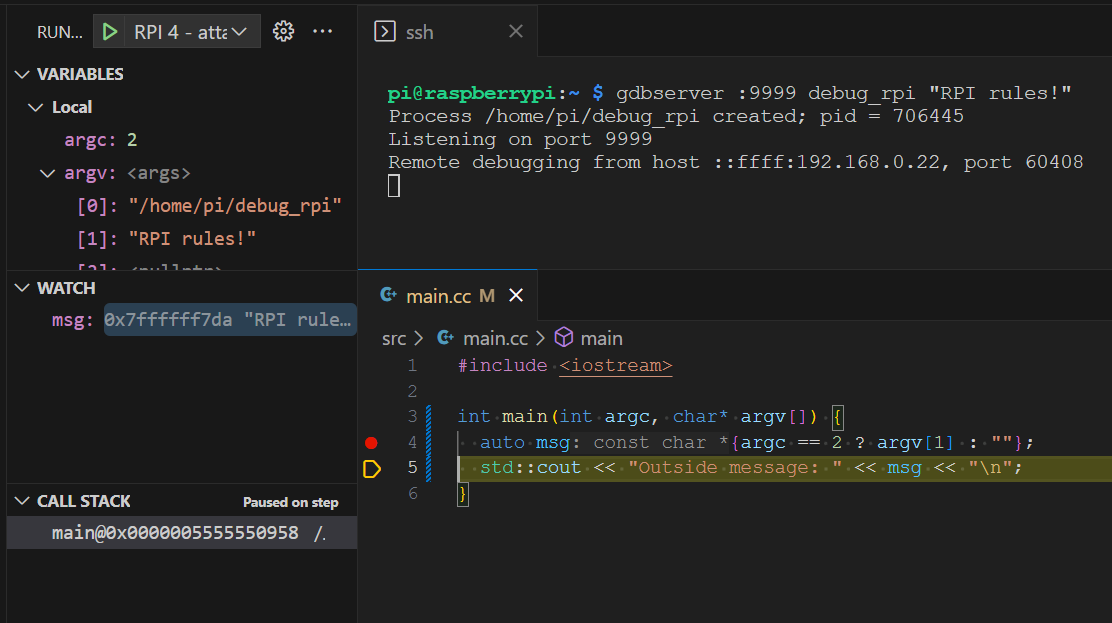
\includegraphics[width=\linewidth]{res/remote_debug_rpi.png}
  % \caption{A boat.}
  \label{fig:debug}
\end{figure}


% Most of the article must be written in a font not smaller than 9pt.
% This article is written with the \fsize.
% {\small This is an example 9pt sentence.}

% However for subscripts, footnotes, etc, you can go at low as 7pt:
% {\scriptsize This is an example \fsize sentence.}

% Feel free to adjust this template in any way you wish!
% The rest of the example contains your generic Lorem ipsum.

\subsection{Tips}


\href{https://github.com/HalfInner/remote_debug_rpi}{Link - Working example} 

\end{document}
